\documentclass[line, margin]{res}
\usepackage{CJK}
\usepackage{url}
\usepackage{graphicx}
\usepackage{wrapfig}

\begin{document}
%\begin{CJK}{GBK}{kai}
\begin{wrapfigure}[0]{r}[0cm]{0.18\textwidth} %this figure will be at the right
%\centering
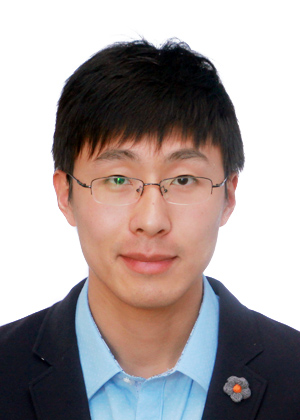
\includegraphics[width=0.18\textwidth]{yang.jpg}
\end{wrapfigure}

\name{Xian Yang}

%\name{����}
\address{No.398 Ruoshui street, industrial district, Suzhou~~~~~~~~~~~~~~~~~~~~~~~}
\address{yangxian10@gmail.com \\ 15952446119~~~~~~~~~~}


%\begin{figure}[!h]
%\raggedleft
%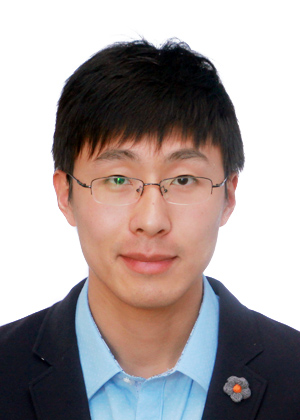
\includegraphics[width=0.18\textwidth]{yang.jpg}
%\end{figure}

\begin{resume}

\section{JOB OBJECTIVE}
\textbf{: Analytics Specialist}

\section{EDUCATION}
%\begin{tabular}{l l l l}
 2010.9 - Present  \textbf{Institute of Semiconductor, CAS} \\
 Doctor of Microelectronics and Solid State Electronics\\

 2006.9 - 2010.7  \textbf{Xidian University}\\
 Bachelor of Applied physics, ranking 1/80
%\end{tabular}

\section{SKILLS}
\begin{itemize}
\item IT skills: \textbf{C/C++}, \textbf{python}, \textbf{matlab}
\item Open source tools: \textbf{OpenCV}, \textbf{scikit-learn}
\item Research interests: \textbf{machine learning, pattern recognition, computer vision}, \textbf{unspecified visual object tracking}
\item Techblog: \url{http://blog.csdn.net/yang_xian521} Page View: \textbf{810,000}
\item CET-6 Pass, excellent reading and writing, basic spoken English
\end{itemize}

\section{EXPERIENCE}
\textbf{Wave Group Intelligent active security R\&D center} \hfill 2012.3-2014.4 \\
\begin{itemize}
\item Designed and optimized unspecified visual tracking algorithm independently, implemented dynamic background unspecified object tracking system robustly.
\item Participated in designing and discussion of single sample person recognition system, achieved 93\% recognition rate in the actual conditions.
\end{itemize}

\textbf{National Undergraduate Electronic Design Contest} \hfill 2009.4-2009.9 \\
\begin{itemize}
\item Established and managed a team of 3 people, took part in internal training and competition
\item Made more than ten electronic modules such as switched-mode power supply, audio power amplifier and CNC obstacle avoidance car, involved the knowledge of digital signal processing, microcontroller programming and analog electronic circuit design.
\item In final match of four days, designed and implemented a digital filter with MCU and FPGA. I managed the organizational scheme and arranged the tasks of each stage.
\end{itemize}

\section{HONORS}
\begin{tabular}{l l l}
Academic�� & 2009 & \textbf{\textit{National Scholarship}(1\%)} \\ [5pt]
 & 2009 & \textbf{\textit{NUEDC Shanxi provincial second prize}} \\ [5pt]
 & 2008 & \textit{Outstanding students pacesetter cadres} \\ [10pt]
Community�� & 2010 & \textbf{\textit{Graduate for outstanding student cadres}(1\%)} \\ [5pt]
 & 2011 & \textbf{\textit{Merit student of CAS.}(2\%)} \\ [5pt]
 & 2007,2009 & \textit{Excellent cyl cadres} \\ [5pt]
 & 2013 & \textit{Outstanding volunteers} \\ [10pt]
Sports�� & & \textit{Prize in the school basketball game for many times}
\end{tabular}

\end{resume}
%\end{CJK}
\end{document}
